\chapter{Analisis}
\label{chap:analisis}


Pada bab ini akan dilakukan analisis mengenai pembuatan model pertumbuhan wirausaha dengan Cellular Automata. Pembahasan akan dimulai dari analisa pertumbuhan wirausaha di Indonesia yang menjadi pokok permasalahan. Lalu dari analisis ini akan dilanjutkan dengan analisis kebutuhan perangkat lunak agar mampu memodelkan pertumbuhan wirausaha di Indonesia.

\section{Analisis Pertumbuhan Wirausaha}
\label{sec:analisisPertumbuhanWirausaha}

Seperti yang sudah dijelaskan pada bab \ref{chap:teori} kewirausahaan dalam negara berkembang seperti Indonesia memang sangat diperlukan untuk membantu meningkatkan pertumbuhan ekonomi. GEM melakukan penelitiannya berdasarkan :
\begin{enumerate}
	\item Keadaan ekonomi negara,
	\item Kemampuan dan motivasi individu serta cara pandang masyarakat mengenai wirausaha,
	\item Pertumbuhan kewirausahaan dan persaingan antar negara tentang seberapa inovatif usaha tersebut.
\end{enumerate}  

Kewirausahaan menurut GEM merupakan sebuah proses yang memiliki tahapan-tahapan yang berbeda. Tahapan yang pertama yaitu individu yang bisa melihat peluang baik dalam berwirausaha dan memiliki kemampuan untuk berwirausaha (\textit{potential entrepreneur}). Kedua, individu yang sudah menjalankan usahanya dalam waktu kurang dari tiga bulan (\textit{nascent entrepreneur}). Ketiga, individu yang sudah menjalankan usahanya selama lebih dari tiga bulan tetapi tidak lebih dari tiga setengah tahun (\textit{new business manager}). Keempat, individu yang sudah menjalankan usahanya lebih dari tiga setengah tahun (\textit{established entrepreneur}). Penjelasan lebih lanjut dapat dilihat pada gambar \ref{fig:prosesWirausaha}. Digunakan \textit{new\_bm} untuk new business manager dan \textit{est\_bm} untuk established business. 

\begin{figure} [H]
	\centering  
	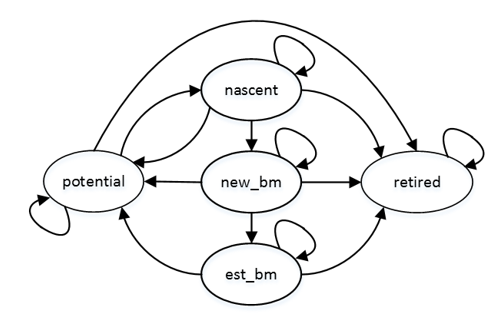
\includegraphics[width=14cm, height=7cm]{tingkatwirausaha} 
	\label{fig:prosesWirausaha} 
\end{figure}


Dalam pertumbuhan wirausaha tentu ada beberapa faktor yang mempengaruhi keberlangsungan pertumbuhan wirausaha. Secara umum, atribut atau faktor yang mempengaruhi pertumbuhan wirausaha yaitu terbagi menjadi 2 jenis yaitu atribut statis dan dinamis. Atribut dinamis yaitu umur, level wirausaha dan usia usaha. Di antara atribut dinamis, level wirausaha menjadi atribut penting karena atribut ini yang akan dijadikan sebagai acuan untuk menentukan perkembangan dari kewirausahaan. Atribut statis yaitu bidang usaha, kategori usaha, jenis kelamin dan lokasi geografis. Sedangkan atribut secara psikologis menurut GEM yaitu Perceived Opportunities, Perceived Capabilities, Entrepreneurial Intention dan Fear of Failure Rate. 


\section{Analisis Pemodelan Cellular Automata}
\label{analisisCA}
Pada penelitian ini akan menggunakan cellular automata berbasis graf. Hal ini dikarenakan jumlah wirausaha di Indonesia yang tidak sedikit, sebab jika menggunakan cellular automata satu atau dua dimensi jumlahnya terbatas.

\subsection{Analisis Ruang Sel}
Ruang sel dalam pemodelan ini berupa individu wirausahawan. Individu wirausahawan memiliki beberapa atribut (umum dan psikologis), masing-masing atribut memiliki nilai yang didapat dari data GEM 2013.

\subsection{Analisis Fungsi Transisi}
Fungsi transisi dalam penelitian ini ditentukan oleh : 
\begin{enumerate}
	\item Atribut Umum
		\begin{enumerate}
			\item Umur
			\item Level Wirausaha
			\item Bidang Usaha
			\item Jenis Kelamin
			\item Pendidikan
			\item Pendapatan
			\item Lokasi
		\end{enumerate}
	\item Atribut Psikologis
		 \begin{enumerate}
			\item Perceived Opportunities
			\item Perceived Capabilities
			\item Role Model
			\item Entrepreneurial of Intention (High Status Successful Entrepreneurship dan Public Media Attention for Entrepreneurship)
			\item Fear of Failure
		 \end{enumerate}
	\item Faktor Publik
		 \begin{enumerate}
			\item Keuangan terkait dengan kewirausahaan
			\item Kebijakan pemerintah terkait ekonomi
			\item Kebijakan pemerintah terkait pajak
			\item Program Pemerintah
			\item Pendidikan kewirausahaan pada SD dan SMP
			\item Pendidikan kewirausahan pada SMK, professional dan universitas
			\item Transfer penelitian dan pengembangan
			\item Infrastruktur komersial dan legal
			\item Keterbukaan Pasar
			\item Norma, Sosial dan Budaya
			\item Infrastruktur Fisik dan Akses Layanan
			\item Dinamika Pasar
		 \end{enumerate}
\end{enumerate}

Selain itu, bobot dari masing-masing ketetanggaan juga mempengaruhi perubahan transisi wirausaha. Perubahan transisi dari individu wirausahawan dapat diketahui melalui angka yang disebut Continuity Index (CIdx).

\begin{displaymath}
\label{RumusCIDx}
	CIdx_{i}(t) = a.Cint_{i}(t) + b.Cneg_{i}(t) + c.Cpub(t)
\end{displaymath}
dimana a,b,c merupakan bilangan riil sedemikian sehingga $0\leq a,b,c \leq 1$ dan $a+b+c=$ 1.0 dan $Cint_{i}(t)$ dan $Cneg_{i}(t)$ melambangkan kondisi internal dan kondisi ketetanggaan dari sebuah individu i pada saat t dan $Cpub(t)$ melambangkan kondisi publik pada saat t nilai dari $CIdx$ dari individu i pada saat t.

CIdx dari seorang wirausahawan ditentukan oleh faktor luar dan dalam. Seorang wirausahawan akan meneruskan usahanya jika CIdx nya memenuhi nilai ambang tersebut. Jika nilai dari Continuity Index sudah sama atau lebih dari nilai ambang, level wirausaha akan berubah. Sebaliknya, jika nilai dari Continuity Index kurang dari sama dengan nilai ambang, level wirausaha bisa saja berubah dan bisa saja tidak berubah.

\section{Analisis Model Pertumbuhan Wirausaha dengan Cellular Automata}
\label{analisismodelCA}

Analisis model pertumbuhan wirausaha bergantung terhadap nilai \textit{Continuity Index} dan nilai ambang (\textit{threshold}). Seperti yang sudah dijelaskan pada \ref{chap:teori}, Continuity Index adalah angka yang menentukan seorang wirausaha akan meneruskan usahanya atau tidak. Sedangkan nilai ambang berfungsi untuk acuan (patokan) perubahan wirausaha dari waktu ke waktu. (Rumus CIDx : \ref{RumusCIDx}).


Nilai dari Continuity Index akan dievaluasi terlebih dahulu menggunakan tabel transisi wirausaha (\ref{tabelLW}). Pada tabel \ref{tabelLW} akan dijelaskan mengenai transisi level dengan menggunakan lambang-lambang \textit{CIdx, bl, a ,b} dan \textit{th} untuk menyatakan \textit{Continuity Index, level} , usia individu, usia usaha dan nilai ambang.


\begin{table}[H]
\centering
\caption{Transisi Level Wirausaha}
\begin{tabular}{|c|c|}
\hline
Waktu sekarang & Waktu berikutnya \\
\hline
\textit{bl} = potential, $ \textit{CIdx} < \textit{th}, \textit{a} < 64 \times 12$ & \textit{bl} = potential \\
\hline
\textit{bl} = potential, $\textit{CIdx} \geq \textit{th}, \textit{a} < 64 \times 12$ & \textit{bl} = nascent \\
\hline
\textit{bl} = potential, $\textit{a} \geq 64 \times 12$ & \textit{bl} = retired \\
\hline
\textit{bl} = nascent, $\textit{CIdx} < \textit{th}, \textit{a} <64 \times 12$ & \textit{bl} = potential \\
\hline
\textit{bl} = nascent, $\textit{CIdx} \geq \textit{th}, \textit{b} < 3$ & \textit{bl} = nascent \\
\hline
\textit{bl} = nascent, $\textit{a} \geq 64 \times 12$ & \textit{bl} = retired \\
\hline
\textit{bl} = new\_bm, $\textit{CIdx} < \textit{th}, \textit{a} < 64 \times 12$ & \textit{bl} = potential \\
\hline
\textit{bl} = new\_bm, $\textit{CIdx} \geq \textit{th}, \textit{b} < 42$ & \textit{bl} = potential \\
\hline
\textit{bl} = new\_bm, $\textit{a} \geq 64 \times 12$ & \textit{bl} = retired \\
\hline
\textit{bl} = est\_bm, $\textit{CIdx} < \textit{th}, \textit{a} < 64 \times 12$ & \textit{bl} = potential \\
\hline
\textit{bl} = est\_bm, $\textit{CIdx} \geq \textit{th}, \textit{a} < 64 \times 12$ & \textit{bl} = est\_bm \\
\hline
\textit{bl} = est\_bm, $\textit{a} \geq 64 \times 12$ & \textit{bl} = retired \\
\hline
\textit{bl} = retired, $\textit{a} \geq 64 \times 12$ & \textit{bl} = retired \\
\hline
\end{tabular}
\label{tabelLW}
\end{table}


Untuk mempermudah pemahaman mengenai Continuity Index, akan diberikan contoh simulasi dari data tidak real, yaitu terdapat nilai a = 0.5, b = 0.4 dan c = 0.1, nilai ambangnya 20, serta periodenya dalam waktu 3 bulan. Nilai dari kondisi internal wirausaha diambil dari Nawangpalupi (Perceived Opportunities = 0.47, Perceived Capabilities = 0.62, High Status of Successful = 0.8, Public Media Attention = 0.75, Role Model = 0.67 dan Fear of Failure = 0.35). Diasumsikan terdapat tiga wirausahawan dan masing-masing wirausahawan memiliki tiga atribut yaitu level wirausaha, umur dan jenis kelamin. Penjelasan lebih lanjut yaitu sebagai berikut :
				
\begin{table} [H]
\centering
\caption{Data wirausahawan}
\begin{tabular}{|c|c|c|c|}
\hline
& Umur & Level Wirausaha & Jenis kelamin\\
\hline
Entrepreneur 1 & 20 tahun & Nascent & Male\\
\hline
Entrepreneur 2 & 35 tahun & New\_bm & Male\\
\hline
Entrepreneur 3 & 44 tahun & New\_bm & Female\\
\hline
\end{tabular}
\end{table}

Berikut data bobot untuk masing-masing atribut :

\begin{table} [H]
\centering
\caption{Data Bobot Atribut}
\begin{tabular}{|c|c|}
\hline
Atribut & Bobot\\
\hline
Umur & 40\% \\
\hline
Jenis Kelamin & 20\% \\
\hline
Level Wirausaha & 40\% \\
\hline
\end{tabular}
\end{table}

	\begin{figure} [H]
		\centering  
		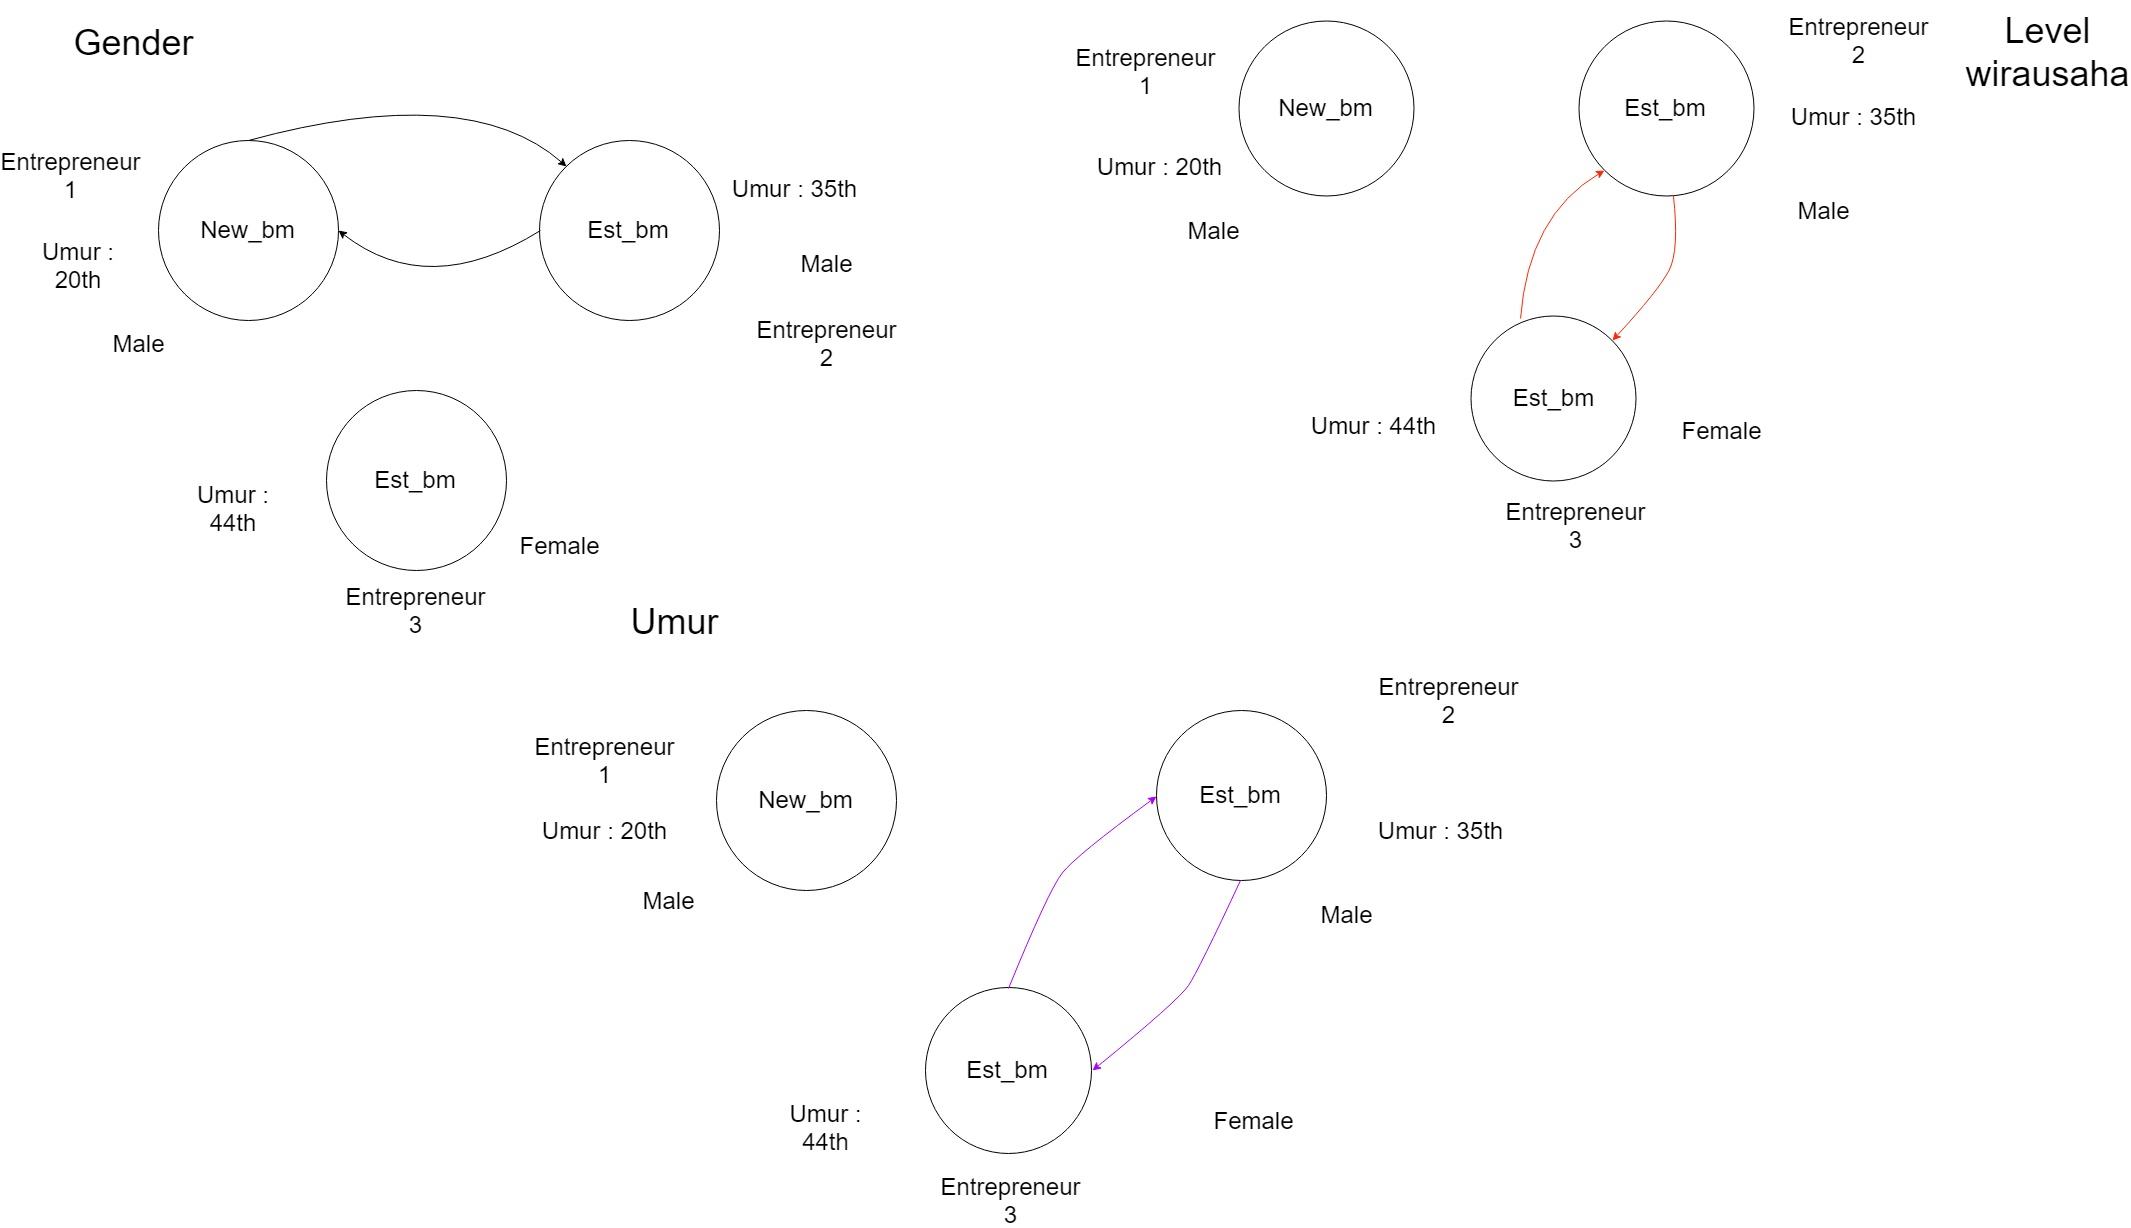
\includegraphics[width=18cm, height=12cm]{wirausahaAwal} 
		\caption[Gambar ketetanggaan tiga entrepreneur pada saat awal]{Gambar ketetanggaan tiga entrepreneur pada saat awal} 
		\label{fig:t0} 
	\end{figure}


Dalam simulasi ini diasumsikan terdapat dua kondisi publik yaitu financial environment related with entrepreneurship yang memiliki nilai 3.06 dan cultural, social norms and society support yang memiliki nilai 3.29, dengan bobot masing-masing 40\% dan 60\%. Perhitungan masing-masing entrepreneur 1, entrepreneur 2 dan entrepreneur 3 (E1,E2,E3) pada saat t=0 yaitu sebagai berikut :
	

\begin{equation}
	CIdx_{1}(t=0) = 0.5 \times ((15.8 \times 0.47) + (15.1 \times 0.62) + (17.1 \times 0.67) + (17 \times 0.8) + (19.5 \times 0.35)) + 0.4 \times ((\frac {1} {2} \times 0.2) + 0 +  0) + 0.1 \times ((3.06 \times 0.4) + (3.29 \times 0.6)) = 24.6948
\end{equation}	

\begin{equation}
	CIdx_{2}(t=0) = 0.5 \times ((28.4 \times 0.47) + (28.2 \times 0.62) + (26.8 \times 0.67) + (26 \times 0.8) + (23.5 \times 0.35)) + 0.4 \times ((\frac {1} {2} \times 0.2) + (\frac {1} {2} \times 0.4) + (\frac {1} {2} \times 0.4)) + (\frac {1} {2} \times 0.4)) + 0.1 \times ((3.06 \times 0.4) + (3.29 \times 0.6)) = 39.4263
\end{equation}

\begin{equation}
	CIdx_{3}(t=0) = 0.5 \times ((28.4 \times 0.47) + (28.2 \times 0.62) + (26.8 \times 0.67) + (26 \times 0.8) + (23.5 \times 0.35)) + 0.4 \times (0 + (\frac {1} {2} \times 0.4) + (\frac {1} {2} \times 0.4)) + 0.1 \times ((3.06 \times 0.4) + (3.29 \times 0.6)) = 39.3863
\end{equation}

	\begin{figure} [H]
		\centering  
		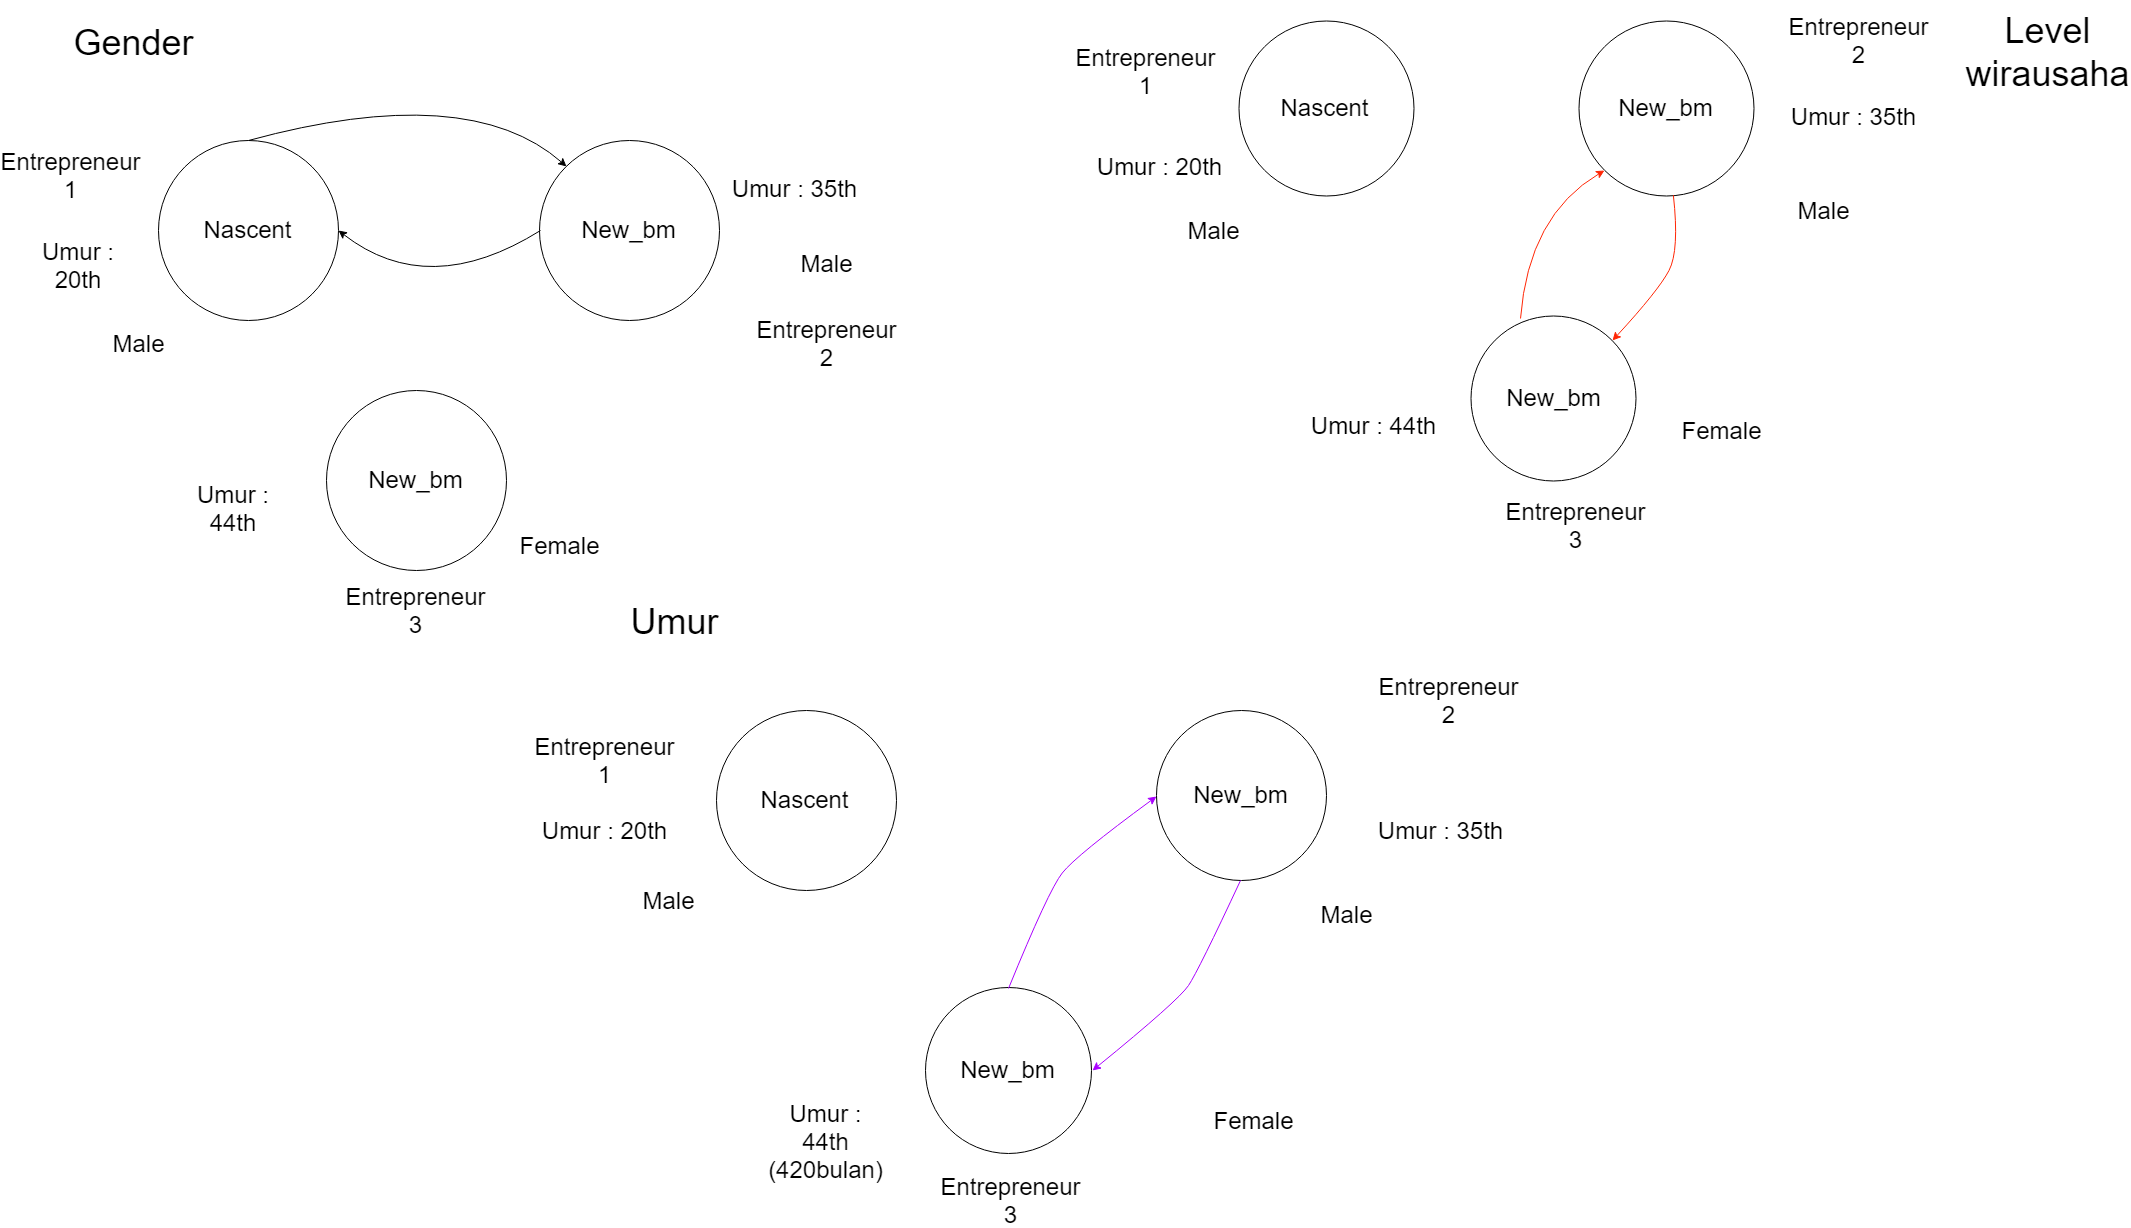
\includegraphics[width=18cm, height=12cm]{wirausaha(t=0)} 
		\caption[Gambar ketetanggaan tiga entrepreneur pada saat t = 0]{Gambar ketetanggaan tiga entrepreneur pada saat t = 0} 
		\label{fig:t0} 
	\end{figure}

Pada saat t=1, Entrepreneur 3 berulang tahun maka umurnya menjadi 45 tahun.

\begin{equation}
	CIdx_{1}(t=1) = 0.5 \times ((15.8 \times 0.47) + (15.1 \times 0.62) + (17.1 \times 0.67) + (17 \times 0.8) + (19.5 \times 0.35)) + 0.4 \times ((\frac {1} {2} \times 0.2) + 0  + 0) + 0.1 \times ((3.06 \times 0.4) + (3.29 \times 0.6)) = 24.6948
\end{equation}

\begin{equation}
	CIdx_{2}(t=1) = 0.5 \times ((28.4 \times 0.47) + (28.2 \times 0.62) + (26.8 \times 0.67) + (26 \times 0.8) + (23.5 \times 0.35)) + 0.4 \times ((\frac {1} {2} \times 0.2) + (\frac {1} {2} \times 0.4) + 0) + 0.1 \times ((3.06 \times 0.4) + (3.29 \times 0.6)) = 39.3463
\end{equation}

\begin{equation}
	CIdx_{3}(t=1) = 0.5 \times ((17.7 \times 0.47) + (16.1 \times 0.62) + (17.6 \times 0.67) + (17 \times 0.8) + (16.4 \times 0.35))+ 0.4 \times (0 + (\frac {1} {2} \times 0.4) + 0) + 0.1 \times ((3.06 \times 0.4) + (3.29 \times 0.6)) = 25.1163
\end{equation}

	\begin{figure} [H]
		\centering  
		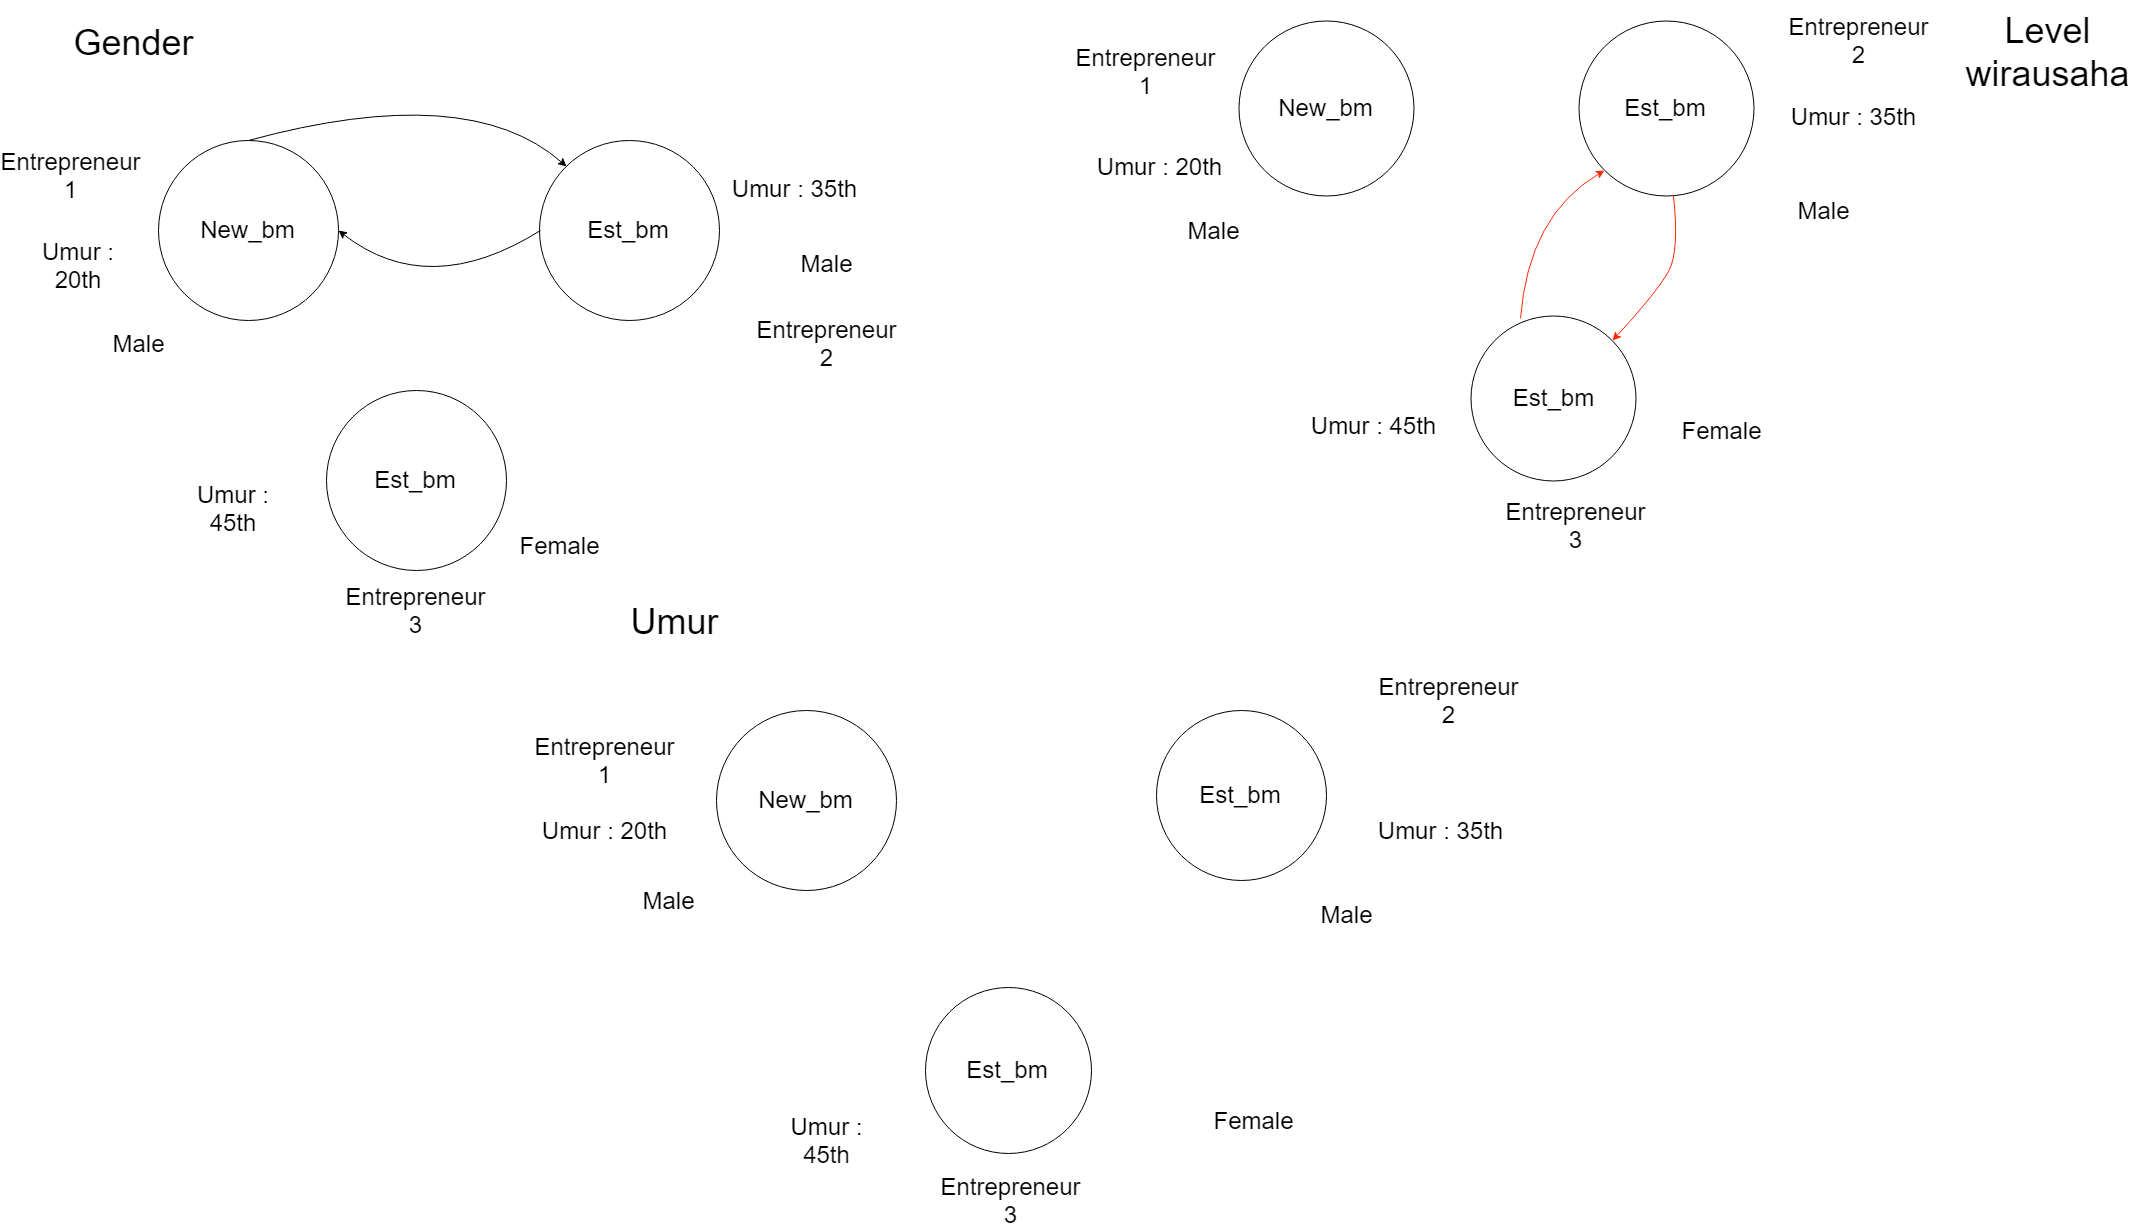
\includegraphics[width=18cm, height=12cm]{wirausaha(t=1)} 
		\caption[Gambar ketetanggaan tiga entrepreneur pada saat t = 1]{Gambar ketetanggaan tiga entrepreneur pada saat t = 1} 
		\label{fig:t0} 
	\end{figure}

Pada saat t=2 terdapat 1 kondisi publik baru yaitu physical infrastructures and services access yang memiliki nilai 3.45 dengan bobot 30\%. Kondisi publik sebelumnya bobotnya menjadi 20\% untuk financial environment related with entrepreneurship, 40\% untuk cultural, social norms and society support.


\begin{equation}
	CIdx_{1}(t=2) =  0.5 \times ((15.8 \times 0.47) + (15.1 \times 0.62) + (17.1 \times 0.67) + (17 \times 0.8) + (19.5 \times 0.35)) + 0.4 \times ((\frac {1} {2} \times 0.2) + 0  + 0) + 0.1 \times ((3.06 \times 0.2) + (3.29 \times 0.4) + (3.45 \times 0.3)) = 25.7298
\end{equation}

\begin{equation}
	CIdx_{2}(t=2) = 0.5 \times ((28.4 \times 0.47) + (28.2 \times 0.62) + (26.8 \times 0.67) + (26 \times 0.8) + (23.5 \times 0.35)) + 0.4 \times ((\frac {1} {2} \times 0.2) + (\frac {1} {2} \times 0.4) + 0) + 0.1 \times ((3.06 \times 0.4) + (3.29 \times 0.6) + (3.45 \times 0.3)) = 40.3813
\end{equation}

\begin{equation}
	CIdx_{3}(t=2) = 0.5 \times ((17.7 \times 0.47) + (16.1 \times 0.62) + (17.6 \times 0.67) + (17 \times 0.8) + (16.4 \times 0.35))+ 0.4 \times (0 + (\frac {1} {2} \times 0.4) + 0) + 0.1 \times ((3.06 \times 0.4) + (3.29 \times 0.6) +(3.45 \times 0.3) ) = 26.1513
\end{equation}

	\begin{figure} [H]
		\centering  
		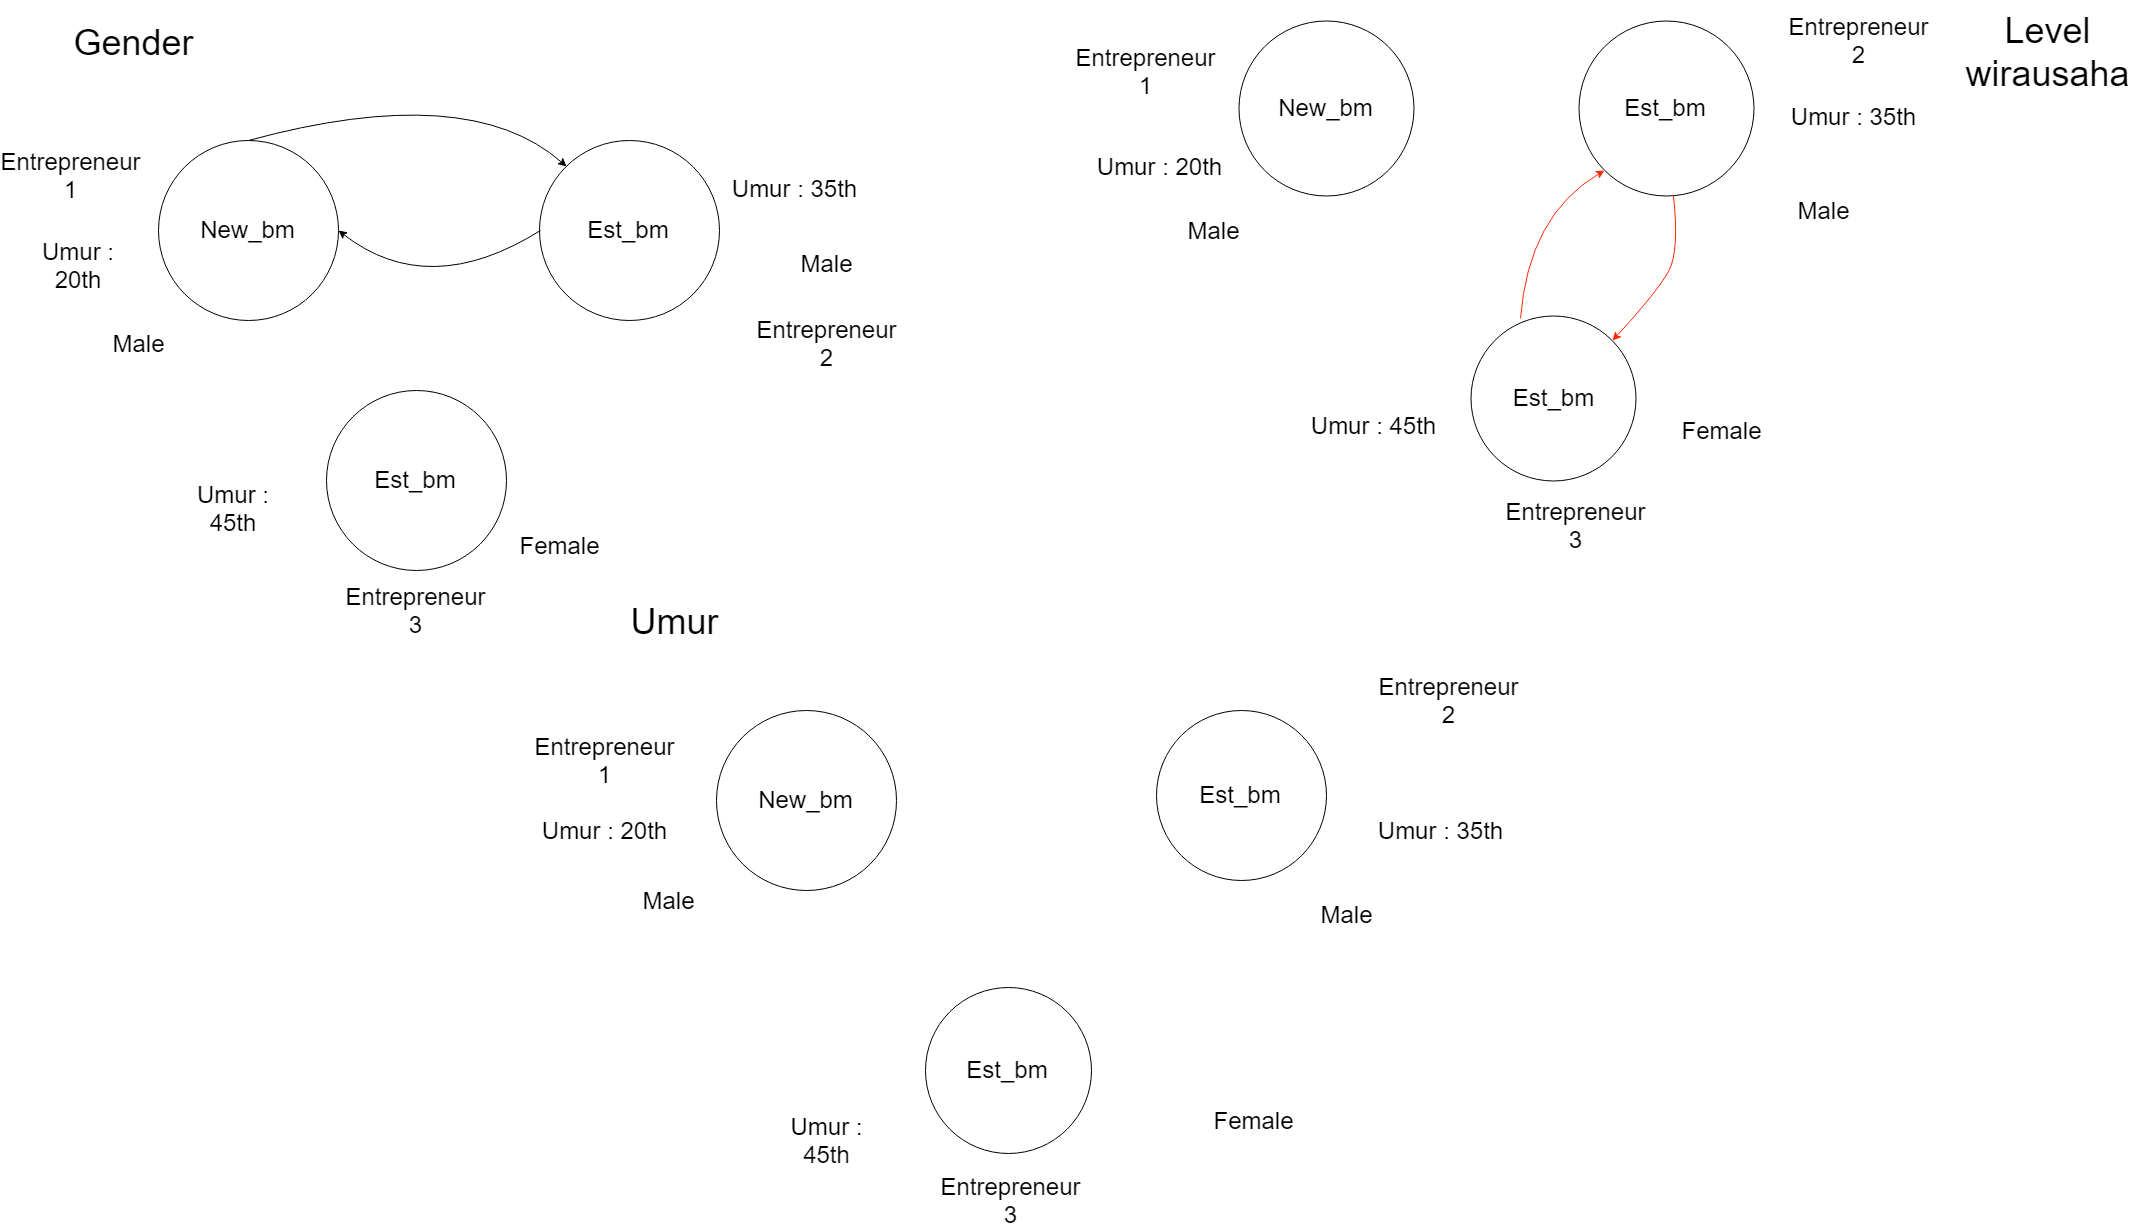
\includegraphics[width=18cm, height=12cm]{wirausaha(t=1)} 
		\caption[Gambar ketetanggaan tiga entrepreneur pada saat t = 2]{Gambar ketetanggaan tiga entrepreneur pada saat t = 2} 
		\label{fig:t0} 
	\end{figure}
	
\section{Deskripsi Perangkat Lunak}
\label{dpl}

Perangkat lunak ini dibuat untuk memberi gambaran kepada pemerintah atau lembaga umum mengenai pergerakkan wirausaha dalam waktu tertentu. Perangkat lunak ini dibangun di netbeans dengan menggunakan \textit{JFrame}. Dalam perangkat lunak ini, disetiap tampilannya terdapat \textit{check box} dan \textit{text field}


\section{Analisis Perangkat Lunak}
\label{analisisPL}

\subsection{Diagram \textit{Use Case}}

Pada diagram \textit{use case} hanya terdapat satu aktor yaitu pemerintah sebagai \textit{user}. Diagram \textit{use case} dapat dilihat pada gambar \ref{fig:usecase}.

	\begin{figure} [H]
		\centering  
		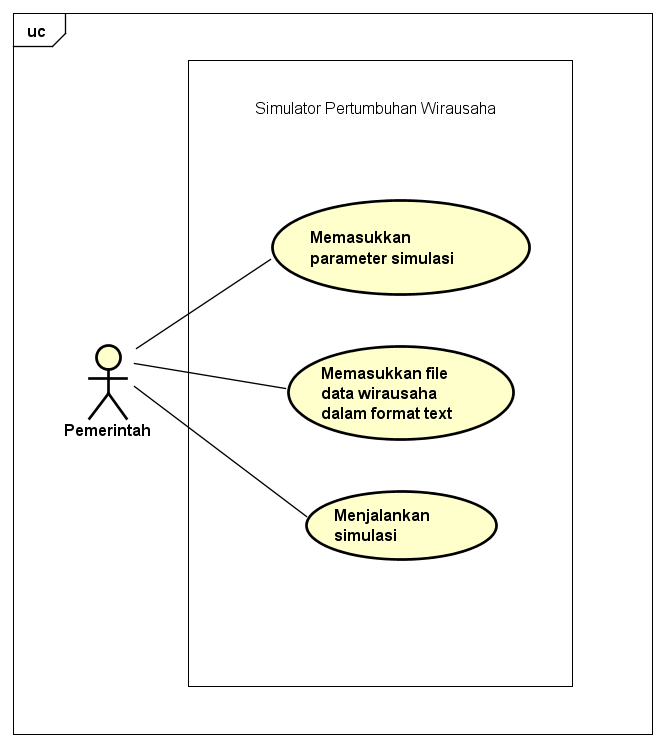
\includegraphics[width=14cm, height=12cm]{UseCase2} 
		\caption[Use Case ECA]{Use Case ECA} 
		\label{fig:usecase} 
	\end{figure}
	
Berdasarkan hasil analisis, dibentuk 3 \textit{use case} dengan 1 aktor, yaitu :
\begin{enumerate}
	\item \textbf{Memasukkan parameter simulasi}
	
	\textit{User} dapat memasukkan parameter seperti bobot setiap ketetanggaan, relasi ketetanggaan, bobot faktor publik, mengisi nilai a,b,c dan threshold serta periode.
	\item \textbf{Memasukkan file data wirausaha dalam format text}
	
	\textit{User} dapat memasukkan data wirausaha yang akan disimulasikan berupa file text.
	\item \textbf{Menjalankan simulasi}
	
	\textit{User} dapat menjalankan simulasi dan melihat hasil simulasi setiap bulannya.
\end{enumerate}

\textbf{Skenario \textit{Use Case}}
\begin{enumerate}
	\item Memasukkan parameter simulasi
	
		\begin{itemize}
			\item Nama : Memasukkan Parameter Simulasi
			\item Aktor : \textit{User}
			\item Deskripsi : Memasukkan bobot untuk setiap atribut dan parameter penting dalam simulasi.
			\item Kondisi awal : \textit{Checkbox} atau \textit{radio button} dan \textit{Text Field} belum terisi.
			\item Kondisi akhir : \textit{User} telah mengisi \textit{checkbox} atau \textit{radio button} dan \textit{text field}.
			\item Skenario utama :
		\end{itemize}
		
\begin{table}[H]
\centering
\caption{Tabel Skenario Memasukkan Parameter Simulasi}
\begin{tabular}{|c|p{7cm}|p{7cm}|}
\hline
No & Aksi & Reaksi Sistem\\
\hline
1 & \textit{User} memasukkan parameter simulasi & Sistem akan menyimpan masukan parameter dari \textit{user}.\\
\hline
\end{tabular}
\label{tabelSkenario1}
\end{table}

	\item Memasukkan File Data Wirausaha Dalam Format Text
	\begin{itemize}
		\item Nama : Memasukkan file data wirausaha dalam format text.
		\item Aktor : \textit{User}.
		\item Deskripsi : Memasukkan file data wirausaha yang akan disimulasikan.
		\item Kondisi awal : \textit{User} meng-klik \textit{button} "OPEN FILE" dan memasukkan file data wirausaha dalam format text.
		\item Kondisi akhir : Sistem akan menampilkan isi data pada tabel.
		\item Skenario utama:
	\end{itemize}
	
	\begin{table}[H]
\centering
\caption{Tabel Skenario Memasukkan file data wirausaha dalam format text}
\begin{tabular}{|c|p{7cm}|p{7cm}|}
\hline
No & Aksi & Reaksi Sistem\\
\hline
1 & \textit{User} meng-klik \textit{button} "OPEN FILE" dan memasukkan file data wirausaha dalam format text. & Sistem akan menampilkan isi data pada tabel. \\
\hline
\end{tabular}
\label{tabelSkenario2}
\end{table}

	\item Menjalankan Simulasi
		\begin{itemize}
			\item Nama : Menjalankan Simulasi
			\item Aktor : \textit{User}
			\item Deskripsi : Menjalankan simulasi dan melihat hasil simulasi
			\item Kondisi awal : \textit{User} meng-klik \textit{button} "SIMULATE"
			\item Kondisi akhir : Sistem akan menampilkan hasil di tabel dan juga di excel.
			\item Skenario utama:
		\end{itemize}
		
\begin{table}[H]
\centering
\caption{Tabel Skenario Menjalankan Simulasi}
\begin{tabular}{|c|p{7cm}|p{7cm}|}
\hline
No & Aksi & Reaksi Sistem\\
\hline
1 & \textit{User} meng-klik \textit{button} "SIMULATE" & Sistem akan menampilkan hasil pada tabel dan juga di excel. \\
\hline
\end{tabular}
\label{tabelSkenario3}
\end{table}
		
\end{enumerate}


\subsection{Diagram Kelas}


Pada bagian ini akan diberikan diagram kelas ECA beserta penjelasannya.

	\begin{figure} [H]
		\centering  
		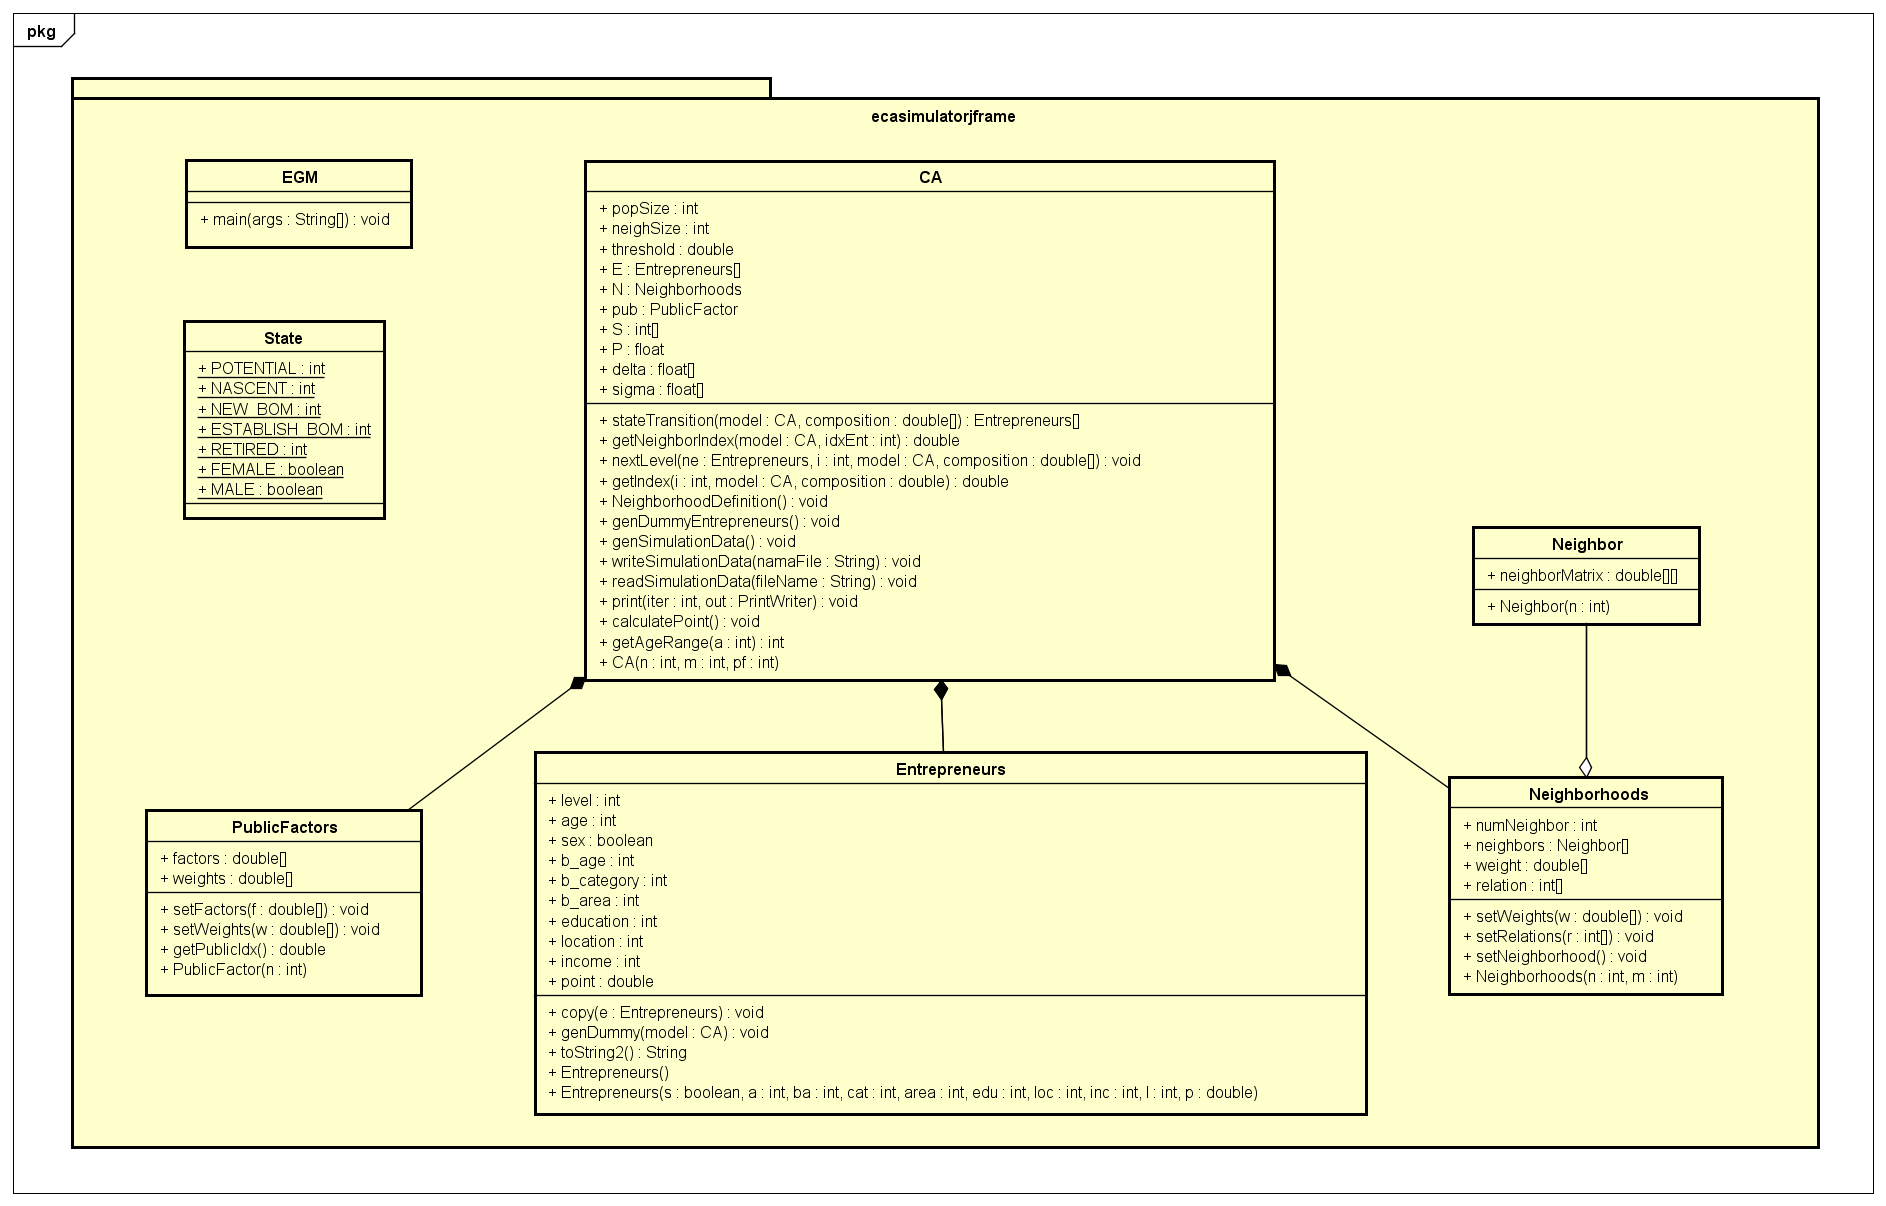
\includegraphics[width=18cm, height=12cm]{diagramKelas0} 
		\caption[Diagram Kelas ECA]{Diagram Kelas ECA} 
		\label{fig:CD1} 
	\end{figure}
	

\subsection{Kelas EGM}
	Kelas EGM merupakan kelas untuk menjalankan perhitungan CIDx, CIDx merupakan angka yang mengindikasikan kemungkinan seorang wirausahawan untuk meneruskan usahanya. Perhitungan CIDx ini menggunakan data dari GEM 2013.
	
\subsection{Kelas CA} 
Kelas CA merupakan kelas yang merepresentasikan cellular automata.
		\begin{enumerate}
			\item 
		\end{enumerate}
		\begin{enumerate}
			\item \texttt{public Entrepreneurs[] stateTransition(CA model, double[] composition)}\\
			Merupakan method untuk menentukan perubahan transisi pada seorang wirausaha yang bergantung pada umur dan nilai ambang.\\			Parameter:
			\begin{itemize}
				\item \texttt{model} merupakan objek dari kelas CA.
				\item \texttt{composition} merupakan nilai a,b dan c.
			\end{itemize}
			
			\item \texttt{public double getNeighborIndex(CA model, int idxEnt)}\\
			Merupakan method untuk menghitung jumlah ketetanggaan antara wirausaha satu dengan wirausaha lainnya.\\
			Parameter:
			\begin{itemize}
				\item \texttt{model} merupakan objek dari kelas CA.
				\item \texttt{idxEnt}
			\end{itemize}
			
			
			\item Method nextLevel
			
			Merupakan method untuk menentukan perubahan level usaha dari seorang wirausaha.
			
			\item Method getIndex
			
			Merupakan method untuk menghitung CIDx.
			
			\item Method NeighborhoodDefinition
			
			Merupakan method untuk mendefinisikan jenis-jenis ketetanggaan seperti lebih dari sama dengan, sama dengan dan lebih kecil sama dengan.
			
			\item Method genDummyEntrepreneurs
			
			Merupakan method untuk membuat data \textit{dummy} wirausaha.
			\item Method genSimulationData
			
			Merupakan method untuk 
			\item Method writeSimulationData
			
			Merupakan method untuk menge-\textit{print} hasil simulasi ke dalam suatu file.
			\item Method readSimulationData
			
			Merupakan method untuk membaca dan memasukkan data file yang akan yang akan disimulasi.
			\item Method print
			\item Method calculatePoint
			
			Merupakan method untuk menghitung kondisi internal dari seorang wirausaha.
			\item Method getAgeRange
			
			Merupakan method untuk membedakan rentang usia yang telah ditentukan oleh GEM 2013.
		\end{enumerate}
\subsection{Kelas Entrepreneur} 
	Kelas Entrepreneur merupakan kelas untuk merepresentasikan individu wirausahawan.
\subsection{Kelas Neighbor}
	Kelas Neighbor merupakan kelas untuk merepresentasikan ketetanggaan untuk satu aspek tertentu. Setiap aspeknya didefinisikan sebagai satu neighbor yang berupa adjacency matrix.
\subsection{Kelas Neighborhood}
	Kelas Neighborhood merupakan kelas untuk merepresentasikan himpunan ketetanggaan yang tersusun atas sejumlah ketetanggaan.
\subsection{Kelas PublicFactor}
	Kelas PublicFactor merupakan kelas untuk merepresentasikan faktok publik.
\subsection{Kelas State}
	Kelas State merupakan kelas untuk memberi nilai untuk setiap level wirausaha.


